\chapter{Performance} 

	\section{Test Setup}
		\subsection{Parameter Space Explored}
		\subsection{Machine Parameters}
		\subsection{Memory Bandwidth Comparison}
	
	\section{Particle list size scan}
The following tests were performed to explore the dependence of sceptic3Dgpu's runtime on the number of particles per node. These tests were performed using two MPI nodes and a grid size of 128x64x64.

\begin{figure}
\begin{center}
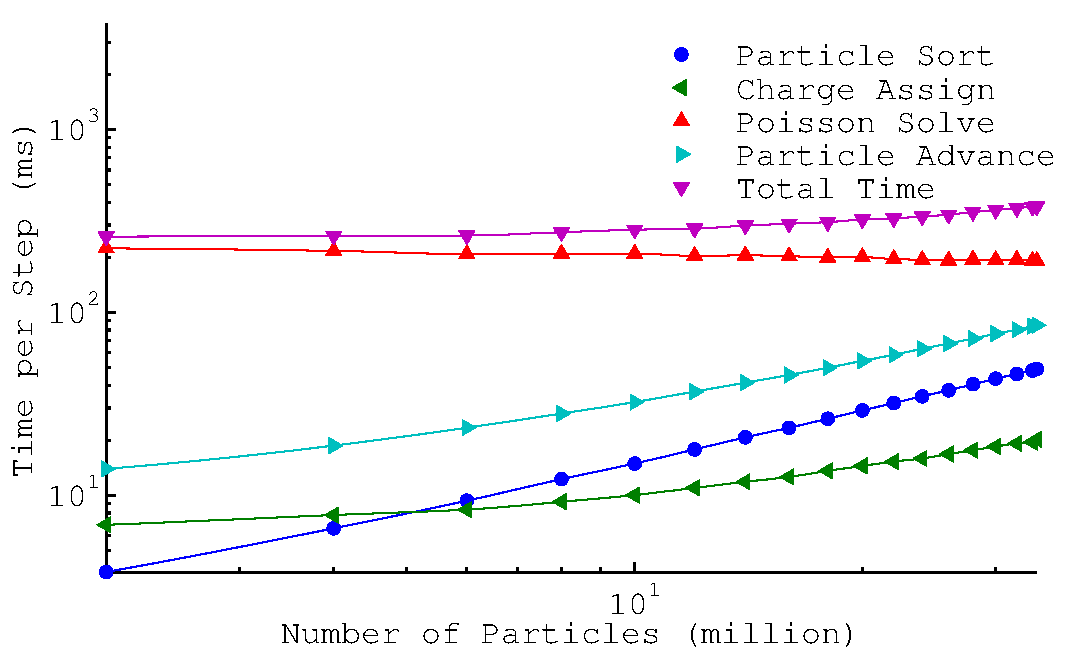
\includegraphics[width=6in]{performance/nptclsize_scan128x64x64ons8bins.pdf}
\end{center}
\caption{Number of Particles Scan on a 128x64x64 grid}
\label{fig:nptclsize_scan128x64x64}
\end{figure}

\begin{figure}
\begin{center}
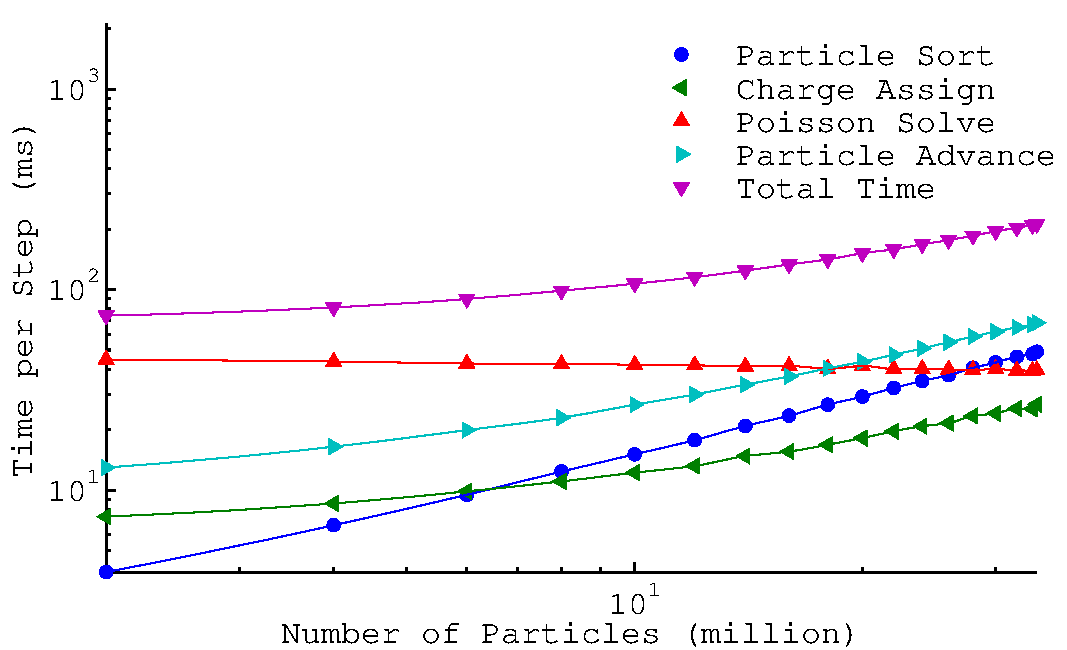
\includegraphics[width=6in]{performance/nptclsize_scan64x32x32ons8bins.pdf}
\end{center}
\caption{Number of Particles Scan on a 64x32x32 grid}
\label{fig:nptclsize_scan128x64x64}
\end{figure}

\begin{figure}
\begin{center}
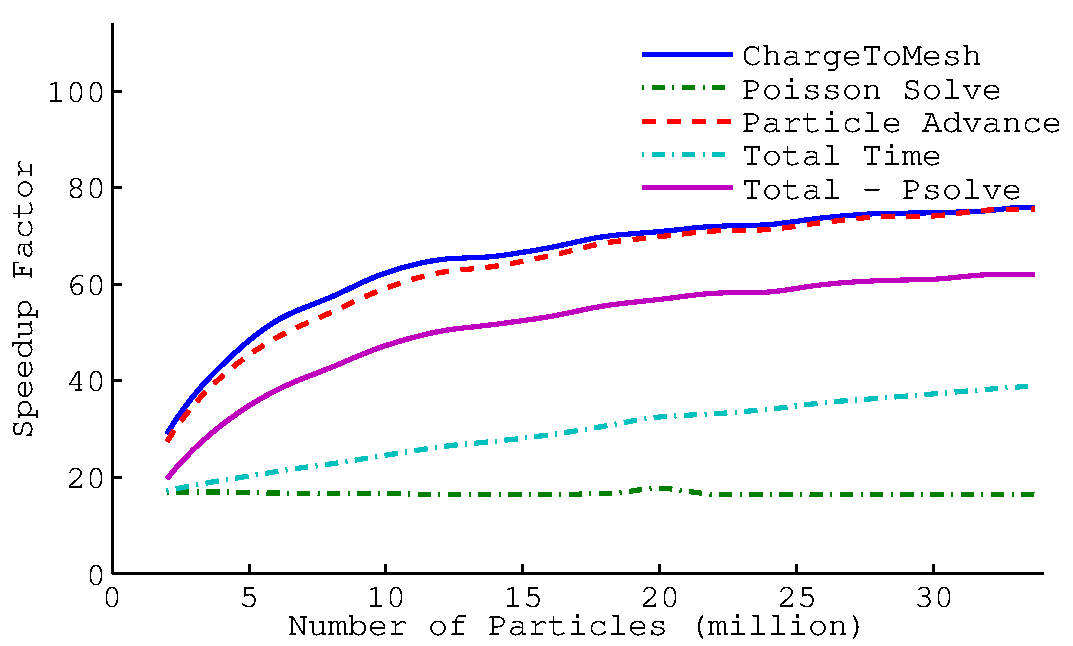
\includegraphics[width=6in]{performance/nptclspeedup_scan128x64x64ons8bins.pdf}
\end{center}
\caption{Speedup factor Number of Particles Scan on a 128x64x64 grid}
\label{fig:nptclsize_scan128x64x64}
\end{figure}


\begin{figure}
\begin{center}
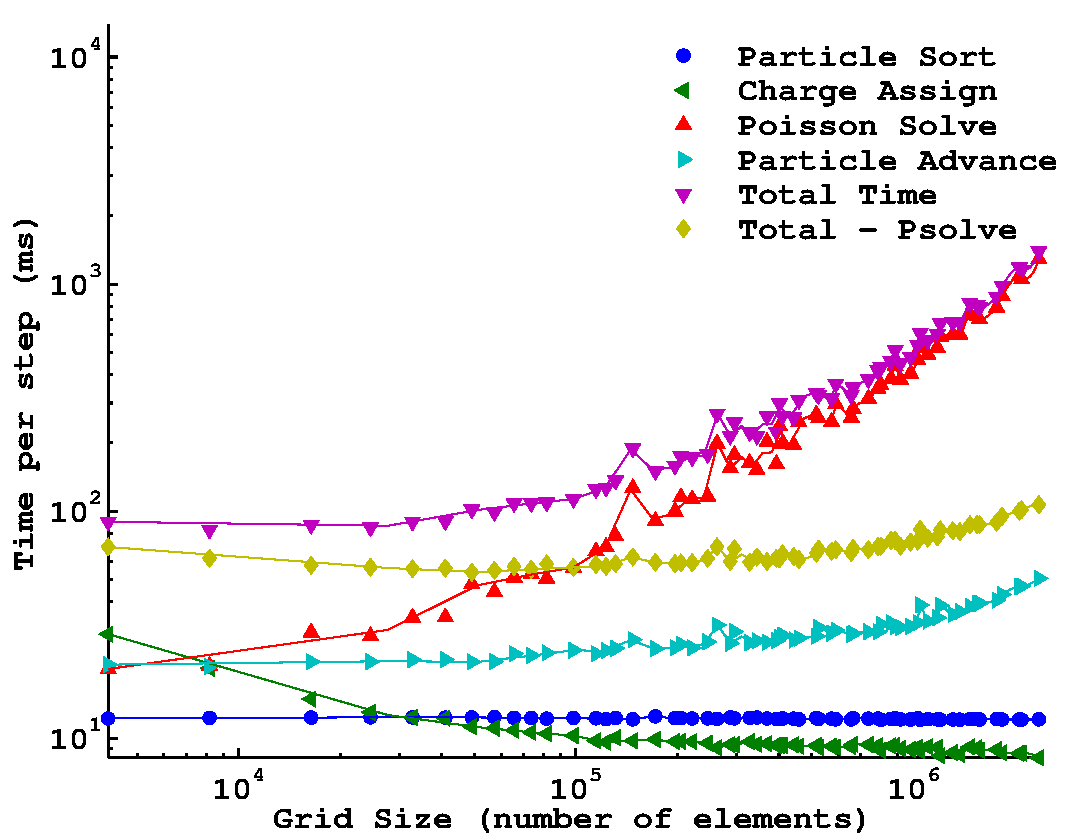
\includegraphics[width=6in]{performance/gridsize_scan8ptcls8bins.pdf}
\end{center}
\caption{Gridsize Scan with 8 million ptcls}
\label{fig:nptclsize_scan128x64x64}
\end{figure}


\begin{figure}
\begin{center}

\includegraphics[width=6in]{performance/gridsize_scan8ptcls16bins.pdf}
\end{center}
\caption{Gridsize Scan with 8 million ptcls}
\label{fig:nptclsize_scan128x64x64}
\end{figure}


\begin{figure}
\begin{center}
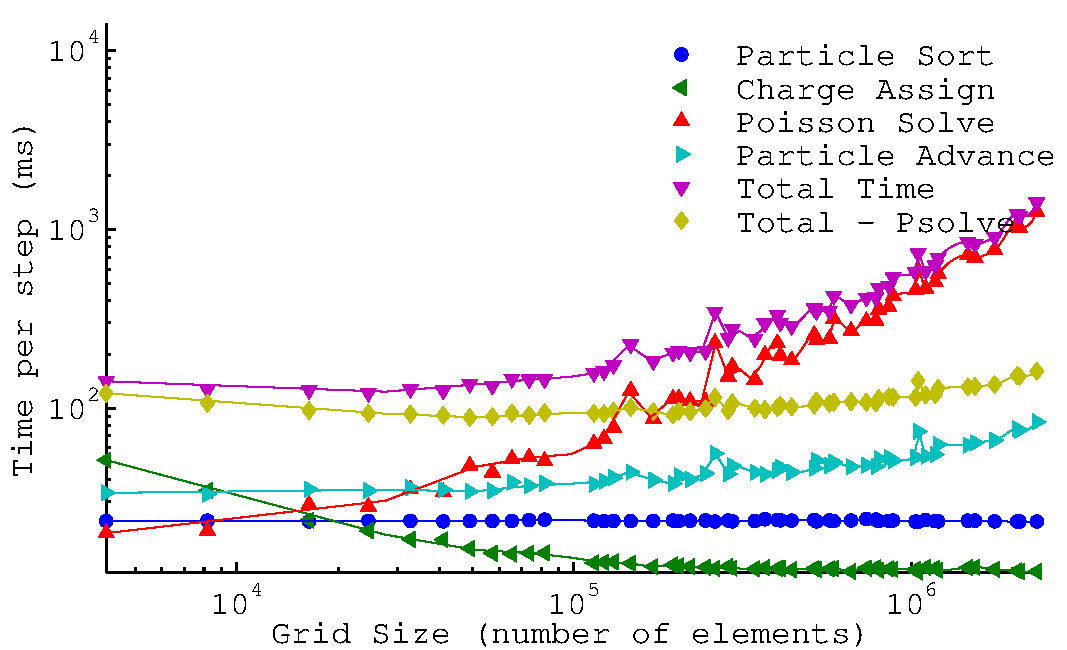
\includegraphics[width=6in]{performance/gridsize_scan16ptcls8bins.pdf}
\end{center}
\caption{Gridsize Scan with 16 million ptcls}
\label{fig:nptclsize_scan128x64x64}
\end{figure}

\begin{figure}
\begin{center}
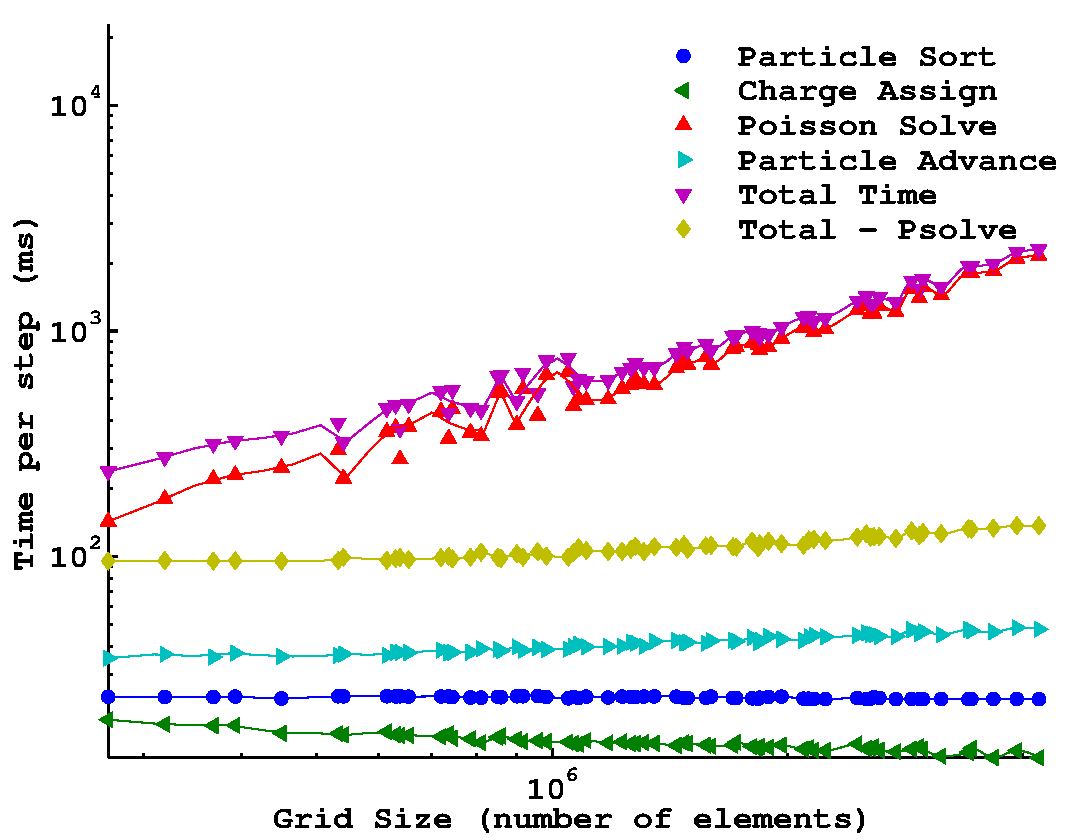
\includegraphics[width=6in]{performance/gridsize_scan16ptcls16bins.pdf}
\end{center}
\caption{Gridsize Scan with 16 million ptcls}
\label{fig:nptclsize_scan128x64x64}
\end{figure}

\begin{figure}
\begin{center}
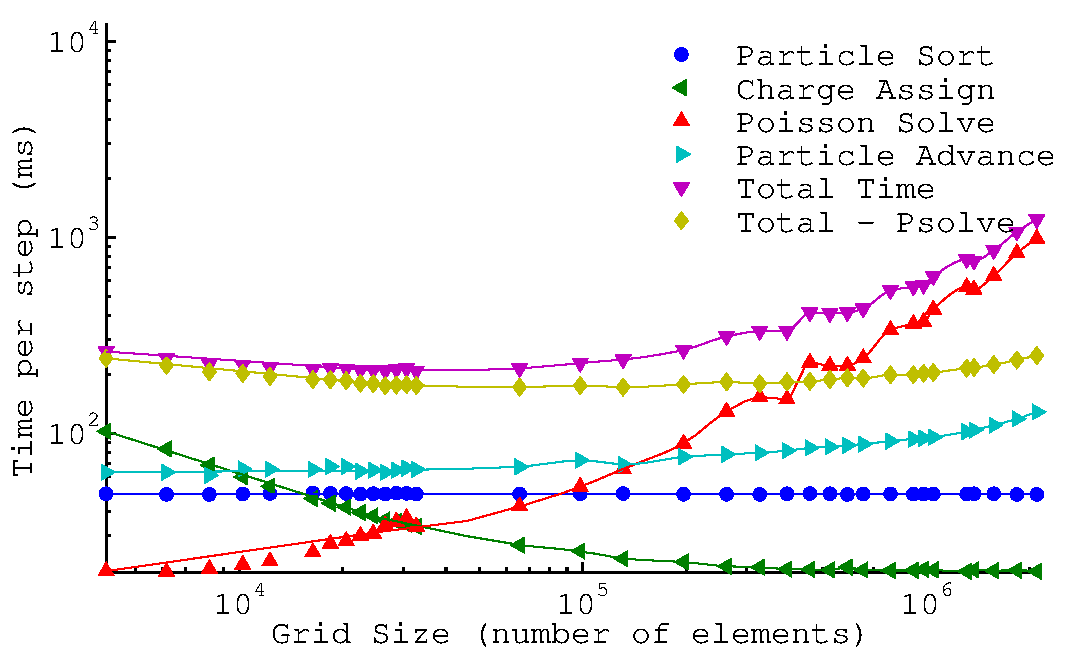
\includegraphics[width=6in]{performance/gridsize_scan34ptcls8bins.pdf}
\end{center}
\caption{Gridsize Scan with 34 million ptcls}
\label{fig:nptclsize_scan128x64x64}
\end{figure}

\begin{figure}
\begin{center}
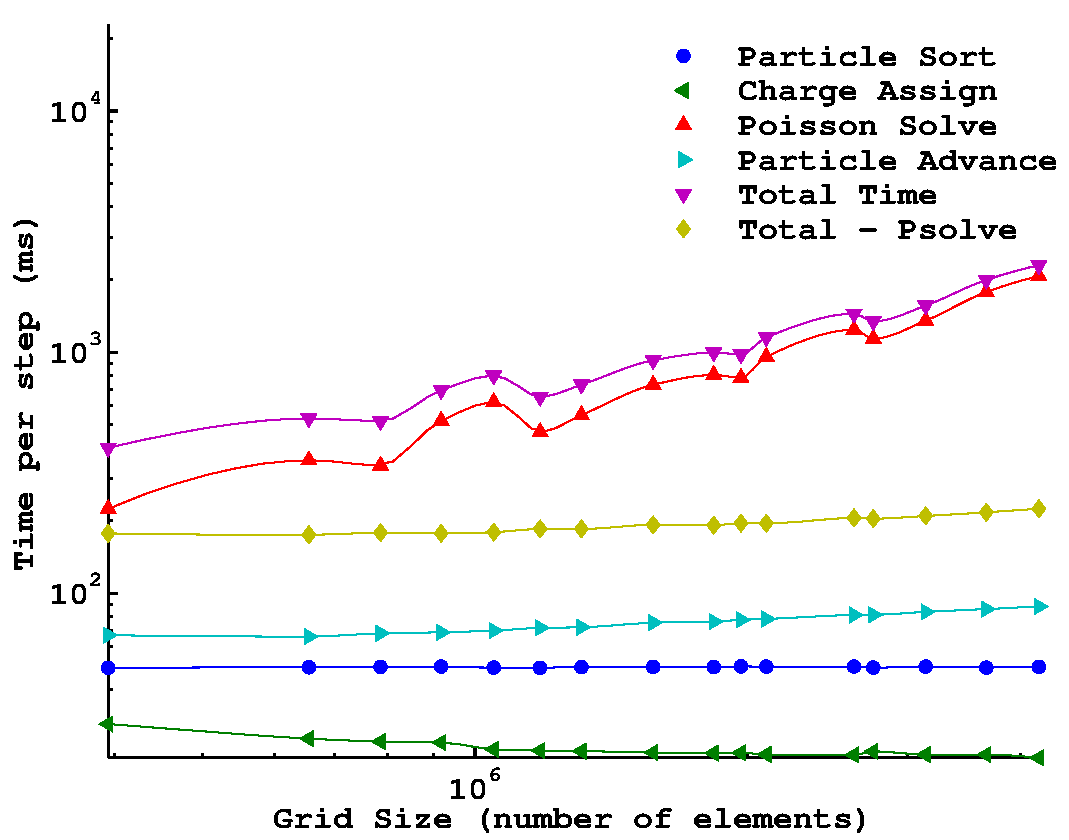
\includegraphics[width=6in]{performance/gridsize_scan34ptcls16bins.pdf}
\end{center}
\caption{Gridsize Scan with 34 million ptcls}
\label{fig:nptclsize_scan128x64x64}
\end{figure}

\begin{figure}
\begin{center}
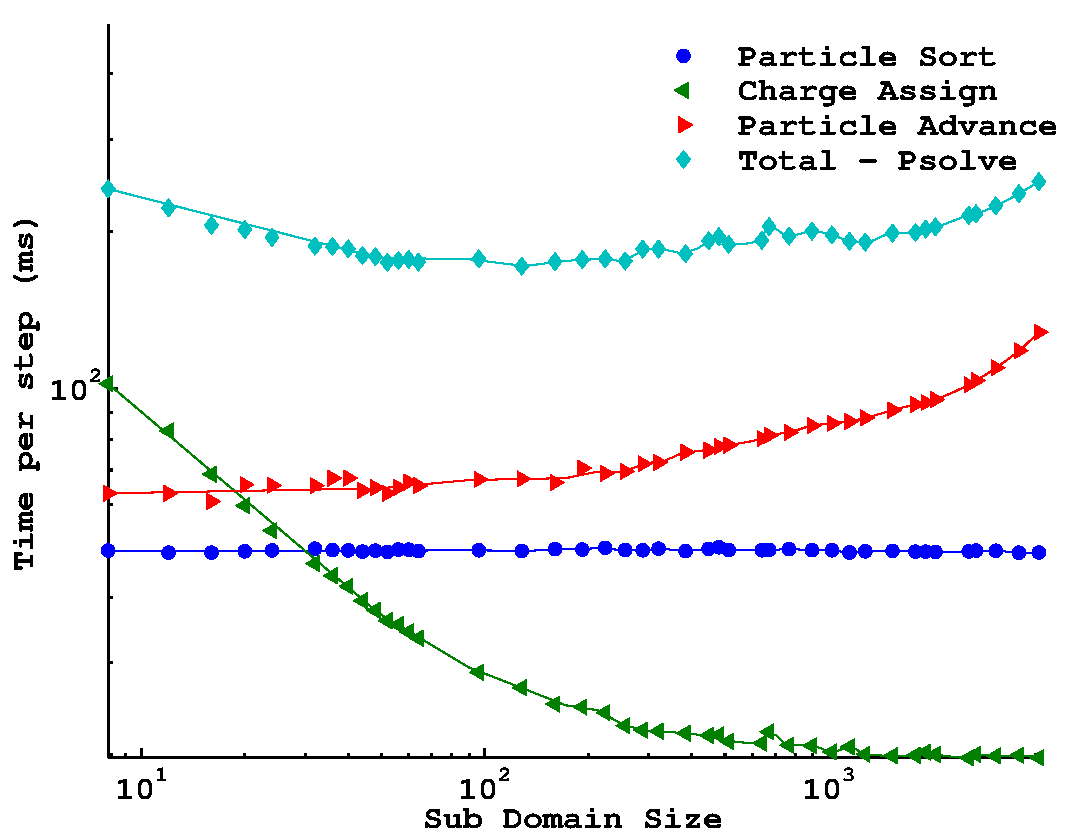
\includegraphics[width=6in]{performance/gridshape_scan.pdf}
\end{center}
\caption{Sub Domain Size scan}
\label{fig:subdomain_size_scan}
\end{figure}

	
	\section{Grid Size scan}
		\subsection{Absolue Size}
		\subsection{Ratio of Surface Area to Volume}
			\subsubsection{Global Domain Ratio}
			\subsubsection{Threadblock Sub-Domain Ratio}

	\section{Kernel Parameters Scan}

	\section{Discussion}
